% Options for packages loaded elsewhere
% Options for packages loaded elsewhere
\PassOptionsToPackage{unicode}{hyperref}
\PassOptionsToPackage{hyphens}{url}
%
\documentclass[
  letterpaper,
]{book}
\usepackage{xcolor}
\usepackage{amsmath,amssymb}
\setcounter{secnumdepth}{5}
\usepackage{iftex}
\ifPDFTeX
  \usepackage[T1]{fontenc}
  \usepackage[utf8]{inputenc}
  \usepackage{textcomp} % provide euro and other symbols
\else % if luatex or xetex
  \usepackage{unicode-math} % this also loads fontspec
  \defaultfontfeatures{Scale=MatchLowercase}
  \defaultfontfeatures[\rmfamily]{Ligatures=TeX,Scale=1}
\fi
\usepackage{lmodern}
\ifPDFTeX\else
  % xetex/luatex font selection
\fi
% Use upquote if available, for straight quotes in verbatim environments
\IfFileExists{upquote.sty}{\usepackage{upquote}}{}
\IfFileExists{microtype.sty}{% use microtype if available
  \usepackage[]{microtype}
  \UseMicrotypeSet[protrusion]{basicmath} % disable protrusion for tt fonts
}{}
\makeatletter
\@ifundefined{KOMAClassName}{% if non-KOMA class
  \IfFileExists{parskip.sty}{%
    \usepackage{parskip}
  }{% else
    \setlength{\parindent}{0pt}
    \setlength{\parskip}{6pt plus 2pt minus 1pt}}
}{% if KOMA class
  \KOMAoptions{parskip=half}}
\makeatother
% Make \paragraph and \subparagraph free-standing
\makeatletter
\ifx\paragraph\undefined\else
  \let\oldparagraph\paragraph
  \renewcommand{\paragraph}{
    \@ifstar
      \xxxParagraphStar
      \xxxParagraphNoStar
  }
  \newcommand{\xxxParagraphStar}[1]{\oldparagraph*{#1}\mbox{}}
  \newcommand{\xxxParagraphNoStar}[1]{\oldparagraph{#1}\mbox{}}
\fi
\ifx\subparagraph\undefined\else
  \let\oldsubparagraph\subparagraph
  \renewcommand{\subparagraph}{
    \@ifstar
      \xxxSubParagraphStar
      \xxxSubParagraphNoStar
  }
  \newcommand{\xxxSubParagraphStar}[1]{\oldsubparagraph*{#1}\mbox{}}
  \newcommand{\xxxSubParagraphNoStar}[1]{\oldsubparagraph{#1}\mbox{}}
\fi
\makeatother


\usepackage{longtable,booktabs,array}
\usepackage{calc} % for calculating minipage widths
% Correct order of tables after \paragraph or \subparagraph
\usepackage{etoolbox}
\makeatletter
\patchcmd\longtable{\par}{\if@noskipsec\mbox{}\fi\par}{}{}
\makeatother
% Allow footnotes in longtable head/foot
\IfFileExists{footnotehyper.sty}{\usepackage{footnotehyper}}{\usepackage{footnote}}
\makesavenoteenv{longtable}
\usepackage{graphicx}
\makeatletter
\newsavebox\pandoc@box
\newcommand*\pandocbounded[1]{% scales image to fit in text height/width
  \sbox\pandoc@box{#1}%
  \Gscale@div\@tempa{\textheight}{\dimexpr\ht\pandoc@box+\dp\pandoc@box\relax}%
  \Gscale@div\@tempb{\linewidth}{\wd\pandoc@box}%
  \ifdim\@tempb\p@<\@tempa\p@\let\@tempa\@tempb\fi% select the smaller of both
  \ifdim\@tempa\p@<\p@\scalebox{\@tempa}{\usebox\pandoc@box}%
  \else\usebox{\pandoc@box}%
  \fi%
}
% Set default figure placement to htbp
\def\fps@figure{htbp}
\makeatother


% definitions for citeproc citations
\NewDocumentCommand\citeproctext{}{}
\NewDocumentCommand\citeproc{mm}{%
  \begingroup\def\citeproctext{#2}\cite{#1}\endgroup}
\makeatletter
 % allow citations to break across lines
 \let\@cite@ofmt\@firstofone
 % avoid brackets around text for \cite:
 \def\@biblabel#1{}
 \def\@cite#1#2{{#1\if@tempswa , #2\fi}}
\makeatother
\newlength{\cslhangindent}
\setlength{\cslhangindent}{1.5em}
\newlength{\csllabelwidth}
\setlength{\csllabelwidth}{3em}
\newenvironment{CSLReferences}[2] % #1 hanging-indent, #2 entry-spacing
 {\begin{list}{}{%
  \setlength{\itemindent}{0pt}
  \setlength{\leftmargin}{0pt}
  \setlength{\parsep}{0pt}
  % turn on hanging indent if param 1 is 1
  \ifodd #1
   \setlength{\leftmargin}{\cslhangindent}
   \setlength{\itemindent}{-1\cslhangindent}
  \fi
  % set entry spacing
  \setlength{\itemsep}{#2\baselineskip}}}
 {\end{list}}
\usepackage{calc}
\newcommand{\CSLBlock}[1]{\hfill\break\parbox[t]{\linewidth}{\strut\ignorespaces#1\strut}}
\newcommand{\CSLLeftMargin}[1]{\parbox[t]{\csllabelwidth}{\strut#1\strut}}
\newcommand{\CSLRightInline}[1]{\parbox[t]{\linewidth - \csllabelwidth}{\strut#1\strut}}
\newcommand{\CSLIndent}[1]{\hspace{\cslhangindent}#1}



\setlength{\emergencystretch}{3em} % prevent overfull lines

\providecommand{\tightlist}{%
  \setlength{\itemsep}{0pt}\setlength{\parskip}{0pt}}



 


% Required packages
\usepackage{graphicx}
\usepackage{geometry}
\usepackage{fancyhdr}
\usepackage{titling}
\usepackage{array}
\usepackage{booktabs}
\usepackage{xcolor}
\usepackage{setspace}
\usepackage{microtype}
% Better integration with Quarto cross-references
\usepackage{hyperref}
\usepackage{cleveref}
\crefformat{section}{Section~#2#1#3}
\crefformat{figure}{Figure~#2#1#3}
\crefformat{table}{Table~#2#1#3}

% Better support for hyperlinks
\usepackage{hyperref}

% % Better support for section references
% \usepackage{nameref}

% % Support for @ in cross-references
% \makeatletter
% \newcommand{\quartoref}[1]{%
%   \@ifundefined{r@#1}{%
%     \textbf{??}%
%   }{%
%     \ref{#1}%
%   }%
% }
% \makeatother

% % Ensure IDs with hyphens work properly
% \newcommand{\hypenref}[1]{\ref{#1}}
% % Callout support
% \usepackage{tcolorbox}
% \tcbuselibrary{skins,breakable}

% Better typography
\usepackage[protrusion=true,expansion=true]{microtype}

% Callout alternative using mdframed
\usepackage{mdframed}
\usepackage{xcolor}

\newenvironment{calloutNote}
  {\begin{mdframed}[backgroundcolor=blue!5,linecolor=blue!75!black,leftmargin=2mm,rightmargin=2mm]}
  {\end{mdframed}}

\newenvironment{calloutTip}
  {\begin{mdframed}[backgroundcolor=green!5,linecolor=green!75!black,leftmargin=2mm,rightmargin=2mm]}
  {\end{mdframed}}

\newenvironment{calloutWarning}
  {\begin{mdframed}[backgroundcolor=orange!5,linecolor=orange!75!black,leftmargin=2mm,rightmargin=2mm]}
  {\end{mdframed}}

% Spacing
\onehalfspacing

% Header and footer styling
\pagestyle{fancy}
\fancyhf{}
\fancyhead[LE,RO]{\slshape\nouppercase{\rightmark}}
\fancyhead[LO,RE]{\slshape\nouppercase{\leftmark}}
\fancyfoot[C]{\thepage}

% % Cross-reference configuration
% \crefformat{section}{Section~#2#1#3}
% \crefformat{figure}{Figure~#2#1#3}
% \crefformat{table}{Table~#2#1#3}

% Custom commands for the affidavit
\newcommand{\titel}{Automating the Modelling of Transformative Artificial Intelligence Risks}
\newcommand{\autor}{Valentin Jakob Meyer}
\newcommand{\myformat}{\today}

% Custom commands for the affidavit
\newcommand{\thesistitle}{Automating the Modelling of Transformative Artificial Intelligence Risks}
\newcommand{\thesisauthor}{Valentin Jakob Meyer}




























% % Required packages
% \usepackage{graphicx}
% \usepackage{geometry}
% \usepackage{fancyhdr}
% \usepackage{titling}
% \usepackage{array}
% \usepackage{booktabs}
% \usepackage{xcolor}
% \usepackage{hyperref}
% \usepackage{setspace}
% \usepackage{microtype}
% \usepackage{tcolorbox}
% \tcbuselibrary{skins,breakable}
% \usepackage{etoolbox}
% \usepackage{cleveref}

% % Better typography
% \usepackage[protrusion=true,expansion=true]{microtype}

% % Spacing
% \onehalfspacing

% % Header and footer styling
% \pagestyle{fancy}
% \fancyhf{}
% \fancyhead[LE,RO]{\slshape\nouppercase{\rightmark}}
% \fancyhead[LO,RE]{\slshape\nouppercase{\leftmark}}
% \fancyfoot[C]{\thepage}

% % Custom commands for the affidavit
% \newcommand{\titel}{Automating the Modelling of Transformative Artificial Intelligence Risks}
% \newcommand{\autor}{Valentin Jakob Meyer}
% \newcommand{\myformat}{\today}  % Or define this to format the date as you prefer

% % Custom commands for the affidavit
% \newcommand{\thesistitle}{Automating the Modelling of Transformative Artificial Intelligence Risks}
% \newcommand{\thesisauthor}{Valentin Jakob Meyer}


% % Callout box styles
% \newtcolorbox{calloutNote}[1][]{
%   enhanced,
%   colback=blue!5!white,
%   colframe=blue!75!black,
%   title=Note,
%   fonttitle=\bfseries,
%   #1
% }

% \newtcolorbox{calloutTip}[1][]{
%   enhanced,
%   colback=green!5!white,
%   colframe=green!75!black,
%   title=Tip,
%   fonttitle=\bfseries,
%   #1
% }

% \newtcolorbox{calloutWarning}[1][]{
%   enhanced,
%   colback=orange!5!white,
%   colframe=orange!75!black,
%   title=Warning,
%   fonttitle=\bfseries,
%   #1
% }
\makeatletter
\@ifpackageloaded{bookmark}{}{\usepackage{bookmark}}
\makeatother
\makeatletter
\@ifpackageloaded{caption}{}{\usepackage{caption}}
\AtBeginDocument{%
\ifdefined\contentsname
  \renewcommand*\contentsname{Table of contents}
\else
  \newcommand\contentsname{Table of contents}
\fi
\ifdefined\listfigurename
  \renewcommand*\listfigurename{List of Figures}
\else
  \newcommand\listfigurename{List of Figures}
\fi
\ifdefined\listtablename
  \renewcommand*\listtablename{List of Tables}
\else
  \newcommand\listtablename{List of Tables}
\fi
\ifdefined\figurename
  \renewcommand*\figurename{Figure}
\else
  \newcommand\figurename{Figure}
\fi
\ifdefined\tablename
  \renewcommand*\tablename{Table}
\else
  \newcommand\tablename{Table}
\fi
}
\@ifpackageloaded{float}{}{\usepackage{float}}
\floatstyle{ruled}
\@ifundefined{c@chapter}{\newfloat{codelisting}{h}{lop}}{\newfloat{codelisting}{h}{lop}[chapter]}
\floatname{codelisting}{Listing}
\newcommand*\listoflistings{\listof{codelisting}{List of Listings}}
\makeatother
\makeatletter
\makeatother
\makeatletter
\@ifpackageloaded{caption}{}{\usepackage{caption}}
\@ifpackageloaded{subcaption}{}{\usepackage{subcaption}}
\makeatother
\usepackage{bookmark}
\IfFileExists{xurl.sty}{\usepackage{xurl}}{} % add URL line breaks if available
\urlstyle{same}
\hypersetup{
  pdftitle={Automating the Modelling of Transformative Artificial Intelligence Risks},
  pdfauthor={Valentin Jakob Meyer},
  hidelinks,
  pdfcreator={LaTeX via pandoc}}


\title{Automating the Modelling of Transformative Artificial
Intelligence Risks}
\author{Valentin Jakob Meyer}
\date{2025-05-26}
\begin{document}
\frontmatter
\maketitle

\renewcommand*\contentsname{Table of contents}
{
\setcounter{tocdepth}{2}
\tableofcontents
}

\mainmatter
\bookmarksetup{startatroot}

\chapter*{Preface}\label{preface}
\addcontentsline{toc}{chapter}{Preface}

\markboth{Preface}{Preface}

This is a Quarto book.

To learn more about Quarto books visit
\url{https://quarto.org/docs/books}.

\bookmarksetup{startatroot}

\chapter*{Abstract}\label{sec-Abstract}
\addcontentsline{toc}{chapter}{Abstract}

\markboth{Abstract}{Abstract}

\bookmarksetup{startatroot}

\chapter*{Outline(s): Table of Contents}\label{sec-ToC}
\addcontentsline{toc}{chapter}{Outline(s): Table of Contents}

\markboth{Outline(s): Table of Contents}{Outline(s): Table of Contents}

\bookmarksetup{startatroot}

\chapter{Introduction}\label{introduction}

\begin{verbatim}
10% of Grade: ~ 14% of text ~ 4200 words ~ 10 pages

-   introduces and motivates the core question or problem
-   provides context for discussion (places issue within a larger debate or sphere of relevance)
-   states precise thesis or position the author will argue for
-   provides roadmap indicating structure and key content points of the essay
\end{verbatim}

\section{Abstract}\label{abstract}

\texttt{{[}x{]}\ \ introduces\ and\ motivates\ the\ core\ question\ or\ problem}

\section{Motivation: Problem
Statement}\label{motivation-problem-statement}

\begin{verbatim}
    AIs are (on the path to) getting smarter than humans
    Humanities (de-centralized) collective information processing, sense-making AND coordination/cooperation is falling behind
    BUT new technology/AI also enables new modes/methods of collective information processing
    therefore this thesis/AMTAIR aspires to be an epistemic tool that enables/empowers humanity (collectively)
\end{verbatim}

\section{Motivation: Research
Question}\label{motivation-research-question}

\texttt{-\ {[}\ {]}\ provides\ context\ for\ discussion\ (places\ issue\ within\ a\ larger\ debate\ or\ sphere\ of\ relevance)}

\section{Scope: Aim \& Context of the
Research}\label{scope-aim-context-of-the-research}

\section{Significance of the Research: Theory of
Change}\label{significance-of-the-research-theory-of-change}

\texttt{-{[}\ {]}\ states\ precise\ thesis\ or\ position\ the\ author\ will\ argue\ for}

\section{Thesis Statement \& Position: (Aim of the
Paper)}\label{thesis-statement-position-aim-of-the-paper}

\texttt{AMTAIR\ is\ a\ new\ epistemic\ tool/framework\ that\ enables/empowers\ humanities\ collective\ information\ processing,\ comprehension\ and\ thereby\ enables\ the\ necessary\ coordination\ ...\ (to\ compete\ with\ AIs?)}

\texttt{{[}\ {]}\ provides\ roadmap\ indicating\ structure\ and\ key\ content\ points\ of\ the\ essay}

\section{Overview: Structure \& Approach of the Paper (Roadmap ---
Theory of
Change)}\label{overview-structure-approach-of-the-paper-roadmap-theory-of-change}

\section{Table of Contents}\label{table-of-contents}

\section{Problem Statement ---
Motivation}\label{problem-statement-motivation}

Continued AI Progress:

\begin{itemize}
\tightlist
\item
  Rapid advancements in AI technology increase both potential benefits
  and risks.
\end{itemize}

Existential Risks (AI X-Risk):

\begin{itemize}
\tightlist
\item
  Advanced AI systems could pose significant threats if misaligned with
  human values.
\end{itemize}

Complexity Challenges:

\begin{itemize}
\tightlist
\item
  The intricate nature of AI systems complicates policy formulation and
  understanding.
\end{itemize}

Limitations of Current Approaches:

\begin{itemize}
\tightlist
\item
  MTAIR's Reliance on Human Labor:

  \begin{itemize}
  \tightlist
  \item
    Modeling Transformative AI Risks (MTAIR) is constrained by manual
    cognitive efforts.\\
  \end{itemize}
\item
  Need for Automation:

  \begin{itemize}
  \tightlist
  \item
    Scaling and automating risk modeling is essential to keep pace with
    AI developments.
  \end{itemize}
\end{itemize}

Opportunity:

\begin{itemize}
\tightlist
\item
  Leveraging new technologies to enhance our ability to model and
  mitigate AI risks.
\end{itemize}

\section{Aim of the Paper}\label{aim-of-the-paper}

\subsection{Research Question \& Scope}\label{research-question-scope}

\subsubsection{Can frontier AI technologies be utilized to automate the
modeling of transformative AI risks, so as to allow for the prediction
of policy
impacts?}\label{can-frontier-ai-technologies-be-utilized-to-automate-the-modeling-of-transformative-ai-risks-so-as-to-allow-for-the-prediction-of-policy-impacts}

Frontier AI Technology: Today's most capable AI systems (e.g.~GPT4 level
LLMs)\\
Scaling Up: Automating the previously ``manual'' cognitive labor\\
Modeling: Formalizing the world views underlying arguments\\
Transformative AI: Level of AI capabilities defined by severe impact on
the world\\
Safety \& Governance Literature: Publications, reports etc. concerned
with risks from AI

Automated Estimation: Non-manual (AI systems + scaffolding), quantified
evaluations\\
Probability Distributions: Formal expressions of the expectations over
future worlds\\
Conditional Trees of Possible Worlds: ``If \ldots{} then\ldots{}''
reasoning over ways things may play out\\
Forecasting Policy Impacts: Qualitative \& quantitative evaluation of
expected outcomes

\subsection{Significance of the
Research}\label{significance-of-the-research}

\section{Theory of Change --- Approach \& Structure of the
Paper}\label{theory-of-change-approach-structure-of-the-paper}

Multiplicative Benefits:

\begin{itemize}
\tightlist
\item
  Automation × Live Prediction Market Integrations × Policy Impact
  Evaluations
\end{itemize}

Explanation:\\
Automation:

\begin{itemize}
\item
  Increases efficiency and scalability of risk modeling.

  Live Prediction Markets:
\item
  Provides up-to-date, collective intelligence to inform models.

  Policy Impact Evaluations:
\item
  Improves the accuracy and relevance of policy assessments.
\end{itemize}

Outcome:

\begin{itemize}
\tightlist
\item
  Enhanced ability to develop effective policies that mitigate AI risks.
\end{itemize}

Visual Aid:

\begin{itemize}
\tightlist
\item
  A diagram illustrating how each component amplifies the others,
  leading to greater overall impact.
\end{itemize}

\subsection{The Coordination Crisis in AI
Governance}\label{the-coordination-crisis-in-ai-governance}

\subsection{1.2 Research Question and
Scope}\label{research-question-and-scope}

\subsection{1.3 The Multiplicative Benefits
Framework}\label{the-multiplicative-benefits-framework}

\subsection{1.4 From Theory to Practice: A
Roadmap}\label{from-theory-to-practice-a-roadmap}

\section{Overview / Table of Contents}\label{overview-table-of-contents}

\bookmarksetup{startatroot}

\chapter{Context}\label{context}

\begin{verbatim}
### 20% of Grade: ~ 29% of text ~ 8700 words ~ 20 pages

- demonstrates understanding of all relevant core concepts

- explains why the question/thesis/problem is relevant in student’s own words (supported by quotations)

- situates it within the debate/course material

- reconstructs selected arguments and identifies relevant assumptions

- describes additional relevant material that has been consulted and integrates it with the course material as well as the research question/thesis/problem
\end{verbatim}

\begin{enumerate}
\def\labelenumi{\arabic{enumi}.}
\tightlist
\item
  successively (chunk my chunk) introduce concepts/ideas --- and 2.
  ground each with existing literature
\end{enumerate}

\section{Background Considerations}\label{background-considerations}

\section{Literature, Concepts \&
Terminology}\label{literature-concepts-terminology}

\subsection{DAG / BayesNets}\label{dag-bayesnets}

\subsection{State of the art (MTAIR) ---
Explanation}\label{state-of-the-art-mtair-explanation}

\subsubsection{Carlsmith Model
(Analytica)}\label{carlsmith-model-analytica}

\section{Theoretical Foundations}\label{theoretical-foundations}

\subsection{\texorpdfstring{\textbf{AI Existential Risk: The Carlsmith
Model}}{AI Existential Risk: The Carlsmith Model}}\label{ai-existential-risk-the-carlsmith-model}

\subsection{\texorpdfstring{\textbf{The Epistemic Challenge of Policy
Evaluation}}{The Epistemic Challenge of Policy Evaluation}}\label{the-epistemic-challenge-of-policy-evaluation}

\subsection{\texorpdfstring{\textbf{Argument Mapping and Formal
Representations}}{Argument Mapping and Formal Representations}}\label{argument-mapping-and-formal-representations}

\subsection{\texorpdfstring{\textbf{Bayesian Networks as Knowledge
Representation}}{Bayesian Networks as Knowledge Representation}}\label{bayesian-networks-as-knowledge-representation}

\subsection{\texorpdfstring{\textbf{The MTAIR Framework: Achievements
and
Limitations}}{The MTAIR Framework: Achievements and Limitations}}\label{the-mtair-framework-achievements-and-limitations}

\subsection{\texorpdfstring{\textbf{``A Narrow Path'': Conditional
Policy Proposals in
Practice}}{``A Narrow Path'': Conditional Policy Proposals in Practice}}\label{a-narrow-path-conditional-policy-proposals-in-practice}

\subsection{(Intro) Example ---
Rain/Sprinkler/Lawn}\label{intro-example-rainsprinklerlawn}

/ Rain/Sprinkler/Lawn DAG / BayesNet --- Extended Example

\begin{verbatim}
…
\end{verbatim}

Own Position/Argument: AMTAIR \ldots{} Own Rain/Sprinkler/Lawn DAG /
BayesNet Implementation

\section{Methodology}\label{methodology}

\subsection{From World Models to Computational
Representation}\label{from-world-models-to-computational-representation}

\subsubsection{Research Design Overview}\label{research-design-overview}

\subsubsection{Formalizing World Models from AI Safety
Literature}\label{formalizing-world-models-from-ai-safety-literature}

\subsubsection{Directed Acyclic Graphs: Structure and
Semantics}\label{directed-acyclic-graphs-structure-and-semantics}

\subsubsection{Quantification Approaches for Probabilistic
Judgments}\label{quantification-approaches-for-probabilistic-judgments}

\subsubsection{Inference Techniques for Complex
Networks}\label{inference-techniques-for-complex-networks}

\subsubsection{Integration with Prediction Markets and Forecasting
Platforms}\label{integration-with-prediction-markets-and-forecasting-platforms}

\section{Practical Real World
Examples}\label{practical-real-world-examples}

MTAIR / Carlsmith Model (Analytica) --- Explanation (--- is motivation:
should come first)

\subsubsection{Kialo}\label{kialo}

\subsubsection{BayeServer}\label{bayeserver}

\subsubsection{BayesNet --- Extended
Example}\label{bayesnet-extended-example}

\subsection{Rain/Sprinkler/Lawn DAG}\label{rainsprinklerlawn-dag}

\subsubsection{Code + documentation}\label{code-documentation}

\begin{figure}

\centering{

\href{https://github.com/VJMeyer/submission}{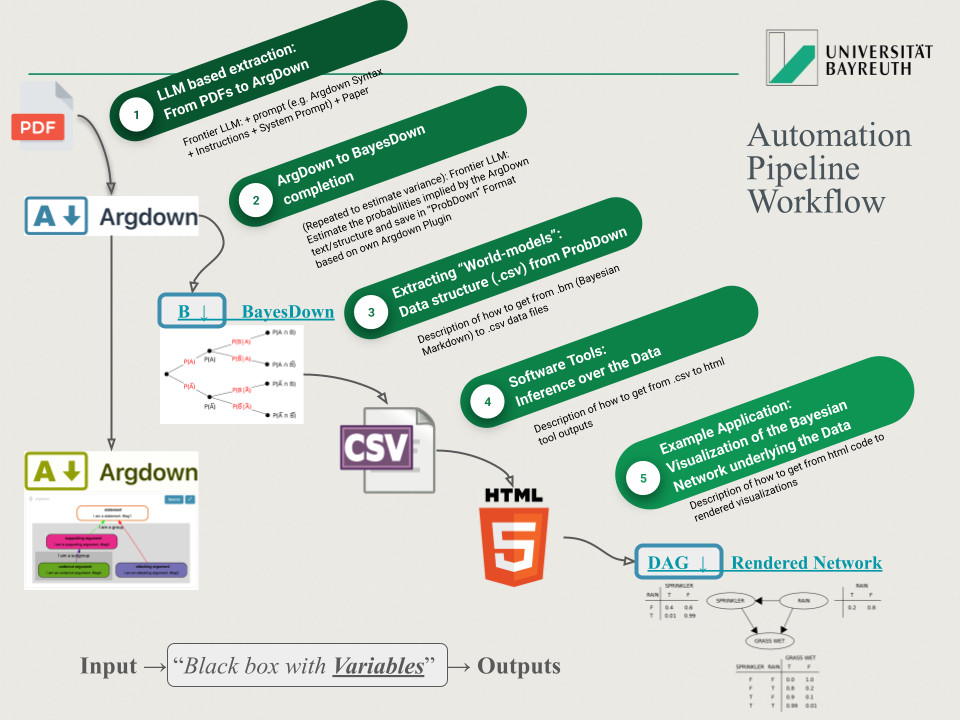
\includegraphics[width=1\linewidth,height=\textheight,keepaspectratio]{images/pipeline.png}}

}

\caption[Five-step AMTAIR automation pipeline from PDFs to Bayesian
networks]{\label{fig-automation_pipeline}AMTAIR Automation Pipeline from
CITATION}

\end{figure}%

Testing crossreferencing grapics Figure~\ref{fig-automation_pipeline}.

\bookmarksetup{startatroot}

\chapter{AMTAIR}\label{amtair}

\begin{verbatim}
### 20% of Grade: ~ 29% of text ~ 8700 words ~ 20 pages

- provides critical or constructive evaluation of positions introduced
- develops strong (plausible) argument in support of author’s own position/thesis
- argument draws on relevant course material claim/argument
- demonstrate understanding of the course materials incl. key arguments and core concepts within the debate
- claim/argument is original or insightful, possibly even presents an original contribution to the debate 
\end{verbatim}

\section{Own Carlsmith Model Implementation ---
Explanation}\label{own-carlsmith-model-implementation-explanation}

\section{Own Implementation: Good example from a published
paper}\label{own-implementation-good-example-from-a-published-paper}

\section{Implementation}\label{implementation}

\subsubsection{System Architecture and Data
Flow}\label{system-architecture-and-data-flow}

\subsubsection{Automated Extraction
Pipeline}\label{automated-extraction-pipeline}

\subsubsection{Network Construction and
Visualization}\label{network-construction-and-visualization}

\subsubsection{Probabilistic Inference
Engine}\label{probabilistic-inference-engine}

\subsubsection{Prediction Market Integration
Module}\label{prediction-market-integration-module}

\subsubsection{Policy Evaluation
Interface}\label{policy-evaluation-interface}

\section{Results: From Theory to
Application}\label{results-from-theory-to-application}

\subsubsection{Extraction Quality
Assessment}\label{extraction-quality-assessment}

\subsubsection{Computational Performance
Analysis}\label{computational-performance-analysis}

\subsubsection{Case Study: The Carlsmith Model
Formalized}\label{case-study-the-carlsmith-model-formalized}

\subsubsection{Comparative Analysis of AI Governance
Worldviews}\label{comparative-analysis-of-ai-governance-worldviews}

\subsubsection{Policy Impact Evaluation: Proof of
Concept}\label{policy-impact-evaluation-proof-of-concept}

TestText

\bookmarksetup{startatroot}

\chapter{Insights \& Findings}\label{insights-findings}

\section{Automated Modeling Pipeline --- From Academic Papers to
Political
Strategy}\label{automated-modeling-pipeline-from-academic-papers-to-political-strategy}

\begin{verbatim}
Success of Automation:
\end{verbatim}

\begin{itemize}
\item
  Demonstrated feasibility of automated model extraction.

  Improved Forecasting:
\item
  Enhanced accuracy with real-time data integration.

  Policy Analysis:
\item
  Identified impactful policies through conditional forecasting.

  Scalability Achieved:
\item
  Efficient processing of extensive data sets.

  Addressed Challenges:
\item
  Overcame limitations of manual modeling.
\end{itemize}

\section{Project Scaling --- Workflow Pipeline \&
Automation}\label{project-scaling-workflow-pipeline-automation}

Scaling Opportunities:

\begin{itemize}
\tightlist
\item
  Horizontal: Incorporate more data sources.\\
\item
  Vertical: Add detailed variables.
\end{itemize}

New Capabilities:

\begin{itemize}
\tightlist
\item
  Advanced analytics.\\
\item
  Real-time data integration.
\end{itemize}

Requirements:

\begin{itemize}
\tightlist
\item
  Software Setup: Robust infrastructure.\\
\item
  Financial: Funding for APIs and compute resources.
\end{itemize}

Impact:

\begin{itemize}
\tightlist
\item
  Broader, more comprehensive models.\\
\item
  Enhanced policy analysis.
\end{itemize}

\section{Computational Complexity --- Computational
Tractability}\label{computational-complexity-computational-tractability}

Challenges:

\begin{itemize}
\tightlist
\item
  High computational demands of complex models.
\end{itemize}

Solutions:

\begin{itemize}
\tightlist
\item
  Clustering Worldviews:\\
\item
  Group similar perspectives to simplify models.\\
\item
  Correlation Management:\\
\item
  Adjust for variable interdependencies.\\
\item
  Efficient Algorithms:\\
  Use optimized sampling methods like Monte Carlo.
\end{itemize}

Outcome:

\begin{itemize}
\tightlist
\item
  Achieved efficiency without sacrificing accuracy.
\end{itemize}

Link to Theory of Change:

\begin{itemize}
\tightlist
\item
  Scalability amplifies policy impact.
\end{itemize}

\section{External Validation --- Manual Extraction \&
Processing}\label{external-validation-manual-extraction-processing}

\begin{verbatim}
Purpose:
\end{verbatim}

\begin{itemize}
\item
  Assess accuracy of automated methods.

  Comparison:
\item
  Automation Strengths:\\
\item
  Speed, consistency.\\
\item
  Human Strengths:\\
\item
  Nuanced understanding.

  Findings:
\item
  Automation excels in data handling.\\
\item
  Human oversight enhances quality.

  Conclusion:
\item
  Optimal results from combining AI with expert input.
\end{itemize}

\bookmarksetup{startatroot}

\chapter{Discussion}\label{discussion}

\begin{verbatim}
10% of Grade: ~ 14% of text ~ 4200 words ~ 10 pages

- discusses a specific objection to student’s own argument
- provides a convincing reply that bolsters or refines the main argument
- relates to or extends beyond materials/arguments covered in class
\end{verbatim}

\bookmarksetup{startatroot}

\chapter{Discussion --- Exchange, Controversy \&
Influence}\label{discussion-exchange-controversy-influence}

\section{Challenges \& Problems --- Red Teaming Problems, Failures \&
Downsides}\label{challenges-problems-red-teaming-problems-failures-downsides}

\begin{verbatim}
Potential Failures:
\end{verbatim}

\begin{itemize}
\item
  Data Issues: Inaccurate or biased inputs.\\
\item
  Model Limitations: Oversimplifications.\\
\item
  Tech Risks: AI misinterpretations.

  Red Teaming:
\item
  Stress-testing models to find weaknesses.

  Impact on Theory of Change:
\item
  Identifying points of failure strengthens the approach.
\end{itemize}

\section{Implications \& Impact --- Uptake, Feedback Loops, Uptake \&
Success -- Green Teaming
--}\label{implications-impact-uptake-feedback-loops-uptake-success-green-teaming}

\begin{verbatim}
Potential Outcomes:
\end{verbatim}

\begin{itemize}
\item
  First-Order: Reduced AI risks through better policies.\\
\item
  Second-Order: Enhanced collaboration.\\
\item
  Third-Order: Framework applied to other global risks.

  Feedback Loops:
\item
  Continuous model improvement.\\
\item
  Adaptive policy-making.

  Green Teaming:
\item
  Strategies to maximize positive impacts.
\end{itemize}

\section{Known Unknowns \& Unknown Unknowns --- Input Data Example:
Modeling Author Worldviews from Bibliographies Instead of Individual
Papers}\label{known-unknowns-unknown-unknowns-input-data-example-modeling-author-worldviews-from-bibliographies-instead-of-individual-papers}

\begin{verbatim}
Potential Outcomes:
\end{verbatim}

\begin{itemize}
\item
  First-Order: Reduced AI risks through better policies.\\
\item
  Second-Order: Enhanced collaboration.\\
\item
  Third-Order: Framework applied to other global risks.

  Feedback Loops:
\item
  Continuous model improvement.\\
\item
  Adaptive policy-making.

  Green Teaming:
\item
  Strategies to maximize positive impacts.
\end{itemize}

\section{Discussion: Implications and
Limitations}\label{discussion-implications-and-limitations}

\subsubsection{Red-Teaming Results: Identifying Failure
Modes}\label{red-teaming-results-identifying-failure-modes}

\subsubsection{Enhancing Epistemic Security in AI
Governance}\label{enhancing-epistemic-security-in-ai-governance}

\subsubsection{Scaling Challenges and
Opportunities}\label{scaling-challenges-and-opportunities}

\subsubsection{Integration with Existing Governance
Frameworks}\label{integration-with-existing-governance-frameworks}

\subsubsection{Known Unknowns and Deep
Uncertainties}\label{known-unknowns-and-deep-uncertainties}

\bookmarksetup{startatroot}

\chapter{Conclusion}\label{conclusion}

\section{The Current State of Things \& How to
Continue}\label{the-current-state-of-things-how-to-continue}

\begin{verbatim}
10% of Grade: ~ 14% of text ~ 4200 words ~ 10 pages

- summarizes thesis and line of argument 
- outlines possible implications
- notes outstanding issues / limitations of discussion
- points to avenues for further research
- overall conclusion is in line with introduction
\end{verbatim}

\section{Summary --- Key Takeaways \&
Findings}\label{summary-key-takeaways-findings}

\subsection{Assessing Policy Effects:}\label{assessing-policy-effects}

Evaluating how different policies alter P(Doom).

\subsection{Conditional Probability:}\label{conditional-probability}

Calculating P(Doom \textbar{} Policy Alpha).

\subsection{Methodology:}\label{methodology-1}

Update model parameters based on policy implementation.

Recompute probabilities accordingly.

\subsection{Purpose:}\label{purpose}

Inform policymakers of potential policy effectiveness.

Prioritize interventions that significantly reduce risks.

\section{Outlook --- Outlook \& Next Steps / Further
Research}\label{outlook-outlook-next-steps-further-research}

\subsection{Scaling Up:}\label{scaling-up}

\begin{itemize}
\tightlist
\item
  Include more variables and data sources.
\end{itemize}

\subsection{Collaboration:}\label{collaboration}

\begin{itemize}
\tightlist
\item
  Partner with policymakers and researchers.
\end{itemize}

\subsection{Technological
Enhancements:}\label{technological-enhancements}

\begin{itemize}
\tightlist
\item
  Employ advanced AI techniques.
\end{itemize}

\subsection{Potential Impact:}\label{potential-impact}

\begin{itemize}
\tightlist
\item
  Influence global AI governance.
\end{itemize}

\subsection{Limitations of the
Analysis}\label{limitations-of-the-analysis}

\subsection{Policy Implications \&
Recommendations}\label{policy-implications-recommendations}

\subsection{Areas for Future Research}\label{areas-for-future-research}

\subsection{Open Questions --- Central/Remaining Questions \&
Feedback}\label{open-questions-centralremaining-questions-feedback}

\subsubsection{Questions:}\label{questions}

\begin{itemize}
\tightlist
\item
  How can we improve automation accuracy?\\
\item
  What challenges exist in policy implementation?\\
\item
  How do we mitigate AI model biases?\\
\item
  How can interdisciplinary efforts enhance outcomes?
\end{itemize}

\subsubsection{Feedback:}\label{feedback}

\begin{itemize}
\tightlist
\item
  Invite thoughts, critiques, and suggestions.
\end{itemize}

\subsection{Outlook --- Outlook \& Next Steps / Further
Research}\label{outlook-outlook-next-steps-further-research-1}

\section{Conclusion: Toward an Adaptive AI Governance
Framework}\label{conclusion-toward-an-adaptive-ai-governance-framework}

\subsection{Key Contributions and
Findings}\label{key-contributions-and-findings}

\subsection{Limitations of the Current
Implementation}\label{limitations-of-the-current-implementation}

\subsection{Policy Implications and
Recommendations}\label{policy-implications-and-recommendations}

\subsection{Future Research
Directions}\label{future-research-directions}

\subsection{Concluding Reflections}\label{concluding-reflections}

\bookmarksetup{startatroot}

\chapter*{Frontmatter}\label{frontmatter}
\addcontentsline{toc}{chapter}{Frontmatter}

\markboth{Frontmatter}{Frontmatter}

\bookmarksetup{startatroot}

\chapter*{Prefatory Apparatus: Illustrations and Terminology --- Quick
References}\label{prefatory-apparatus-illustrations-and-terminology-quick-references}
\addcontentsline{toc}{chapter}{Prefatory Apparatus: Illustrations and
Terminology --- Quick References}

\markboth{Prefatory Apparatus: Illustrations and Terminology --- Quick
References}{Prefatory Apparatus: Illustrations and Terminology --- Quick
References}

\section*{List of Tables}\label{list-of-tables}
\addcontentsline{toc}{section}{List of Tables}

\markright{List of Tables}

Table 1: Table name

Table 2: Table name

Table 3: Table name

\begin{itemize}
\tightlist
\item
  Figure 1.1: The coordination crisis in AI governance - visualization
  of fragmentation\\
\item
  Figure 2.1: The Carlsmith model - DAG representation\\
\item
  Figure 3.1: Research design overview - workflow diagram\\
\item
  Figure 3.2: From natural language to BayesDown - transformation
  process\\
\item
  Figure 4.1: ARPA system architecture - component diagram\\
\item
  Figure 4.2: Visualization of Rain-Sprinkler-Grass\_Wet Bayesian
  network - screenshot\\
\item
  Figure 5.1: Extraction quality metrics - comparative chart\\
\item
  Figure 5.2: Comparative analysis of AI governance worldviews - network
  visualization\\
\item
  Table 2.1: Comparison of approaches to AI risk modeling\\
\item
  Table 3.1: Probabilistic translation guide for qualitative
  expressions\\
\item
  Table 4.1: System component responsibilities and interactions\\
\item
  Table 5.1: Policy impact evaluation results - summary metrics
\end{itemize}

\section*{List of Graphics \& Figures}\label{list-of-graphics-figures}
\addcontentsline{toc}{section}{List of Graphics \& Figures}

\markright{List of Graphics \& Figures}

\section*{List of Abbreviations}\label{list-of-abbreviations}
\addcontentsline{toc}{section}{List of Abbreviations}

\markright{List of Abbreviations}

esp.~especially

f., ff.~following

incl.~including

p., pp.~page(s)

MAD Mutually Assured Destruction

\begin{itemize}
\tightlist
\item
  AI - Artificial Intelligence\\
\item
  AGI - Artificial General Intelligence\\
\item
  ARPA - AI Risk Pathway Analyzer\\
\item
  DAG - Directed Acyclic Graph\\
\item
  LLM - Large Language Model\\
\item
  MTAIR - Modeling Transformative AI Risks\\
\item
  P(Doom) - Probability of existential catastrophe from misaligned AI\\
\item
  CPT - Conditional Probability Table
\end{itemize}

\section*{Glossary}\label{glossary}

\markright{Glossary}

\begin{itemize}
\tightlist
\item
  \textbf{Argument mapping}: A method for visually representing the
  structure of arguments\\
\item
  \textbf{BayesDown}: An extension of ArgDown that incorporates
  probabilistic information\\
\item
  \textbf{Bayesian network}: A probabilistic graphical model
  representing variables and their dependencies\\
\item
  \textbf{Conditional probability}: The probability of an event given
  that another event has occurred\\
\item
  \textbf{Directed Acyclic Graph (DAG)}: A graph with directed edges and
  no cycles\\
\item
  \textbf{Existential risk}: Risk of permanent curtailment of humanity's
  potential\\
\item
  \textbf{Power-seeking AI}: AI systems with instrumental incentives to
  acquire resources and power\\
\item
  \textbf{Prediction market}: A market where participants trade
  contracts that resolve based on future events\\
\item
  \textbf{d-separation}: A criterion for identifying conditional
  independence relationships in Bayesian networks\\
\item
  \textbf{Monte Carlo sampling}: A computational technique using random
  sampling to obtain numerical results
\end{itemize}

\section*{\texorpdfstring{Checklists }{Checklists }}\label{checklists}
\addcontentsline{toc}{section}{Checklists }

\markright{Checklists }

\section*{``Usual paper requirements''}\label{usual-paper-requirements}
\addcontentsline{toc}{section}{``Usual paper requirements''}

\markright{``Usual paper requirements''}

\begin{itemize}
\tightlist
\item
  introduce all terminology

  \begin{itemize}
  \tightlist
  \item
    go through text, make sure all terms are defined, explained (and
    added to the list of Abbr.) when first mentioned\\
  \end{itemize}
\item
  readership is intelligent and interested but has no prior knowledge
\end{itemize}

\section*{}\label{section}
\addcontentsline{toc}{section}{}

\markright{}

\section*{(Format:) \textasciitilde{} Anything that makes it easier to
understand}\label{format-anything-that-makes-it-easier-to-understand}
\addcontentsline{toc}{section}{(Format:) \textasciitilde{} Anything that
makes it easier to understand}

\markright{(Format:) \textasciitilde{} Anything that makes it easier to
understand}

\begin{itemize}
\tightlist
\item
  short sentences\\
\item
  paragraphs (one idea per paragraph)\\
\item
  simplicity\\
\item
  !limit use of passive voice!\\
\item
  use active voice, even prefer I over we!\\
\item
  minimise use of ``zombi nouns'' (don't turn verbs/adjectives to
  nouns!)\\
\item
  ``find words that can be cut''
\end{itemize}

-- the paper can \textbf{focus} on \textbf{one aspect of the
presentation}

-- ``open door policy'' for (content) questions

\textasciitilde{} demonstrate ability for novel research

-- ``solve research question with the tools accessible to you''

-- ``show something that has not been shown before / should be
publishable in principle''

-- new idea (or criticism) ``in this field''

-- Outline idea THEN reading with a purpose (answering concrete
questions)

-- ``Only'' confirm that nobody has published the exact same idea on the
same topic

-- pretty much determined by presentation \& proposal but narrow down
further (\& choose supervisor?)

\subsection*{Quarto Features Incompatible with LaTeX
(Below)}\label{quarto-features-incompatible-with-latex-below}

\bookmarksetup{startatroot}

\chapter{Quarto Syntax}\label{quarto-syntax}

\section*{Figures}\label{sec-figues}

\markright{Figures}

\begin{figure}

\centering{

\href{https://github.com/VJMeyer/submission}{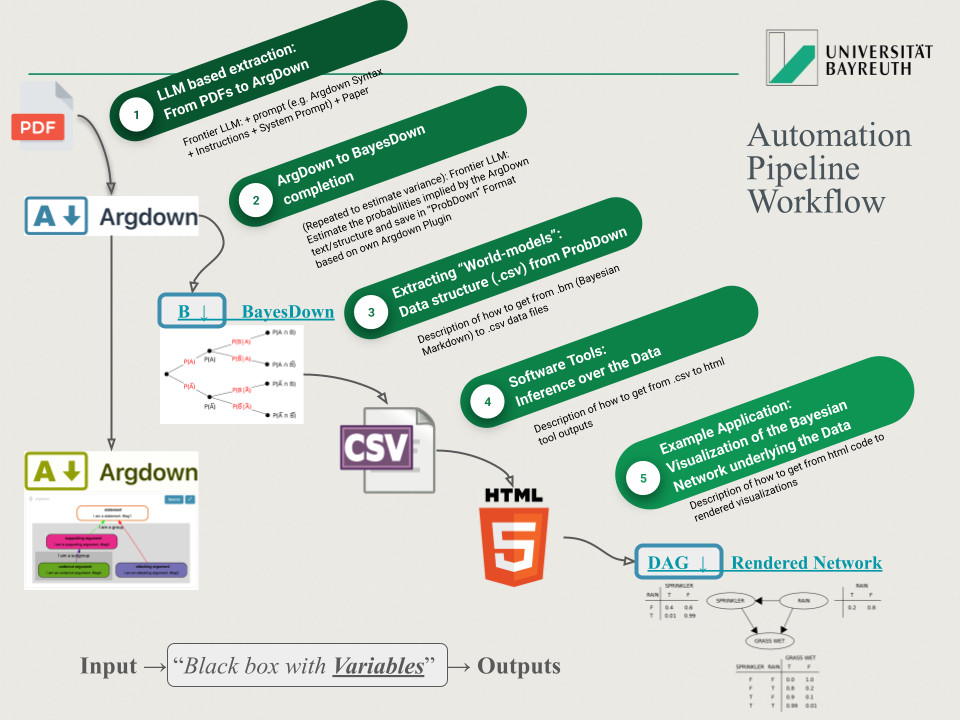
\includegraphics[width=1\linewidth,height=\textheight,keepaspectratio]{images/pipeline.png}}

}

\caption[Five-step AMTAIR automation pipeline from PDFs to Bayesian
networks]{\label{fig-automation_pipeline}AMTAIR Automation Pipeline from
Bucknall and Dori-Hacohen (2022)}

\end{figure}%

Testing crossreferencing grapics Figure~\ref{fig-automation_pipeline}.

\begin{figure}


\includegraphics[width=0.3\linewidth,height=\textheight,keepaspectratio]{images/cover.png}

\caption[Short 2 caption]{\label{fig-testgraphic2}Caption/Title 2}

\end{figure}%

Testing crossreferencing grapics Figure~\ref{fig-testgraphic2}.

\section*{Citations}\label{sec-citations}

\markright{Citations}

Soares and Fallenstein (2014)

(Soares and Fallenstein 2014) and (Knuth 1984)

Blah Blah (see Knuth 1984, 33--35; also Growiec 2024, chap. 1)

Blah Blah (Knuth 1984, 33--35, 38--39 and passim)

Blah Blah (Growiec 2024; Knuth 1984).

Growiec says blah (2024)

\section{Headings \& Potential Headings}\label{sec-heading}

\texttt{verbatim\ code\ formatting\ for\ notes\ and\ ideas\ to\ be\ included\ (here)}

\begin{verbatim}
Also code blocks for more extensive notes and ideas to be included and checklists
- test 1. 
- test 2. 
- test 3.
2. second
3. third
\end{verbatim}

\begin{quote}
Blockquote formatting for ``Suggested Citations (e.g.~carlsmith 2024 on
\ldots)'' and/or claims which require a citation (e.g.~claim x should be
backed-up by a ciation from the literature)
\end{quote}

Here is an inline note.\footnote{Inlines notes are easier to write,
  since you don't have to pick an identifier and move down to type the
  note.}

Here is a footnote reference,\footnote{Here is the footnote.}

\renewcommand*{\labelitemi}{\textgreater}

Here's some raw inline HTML:

page 1

\newpage{}

page 2

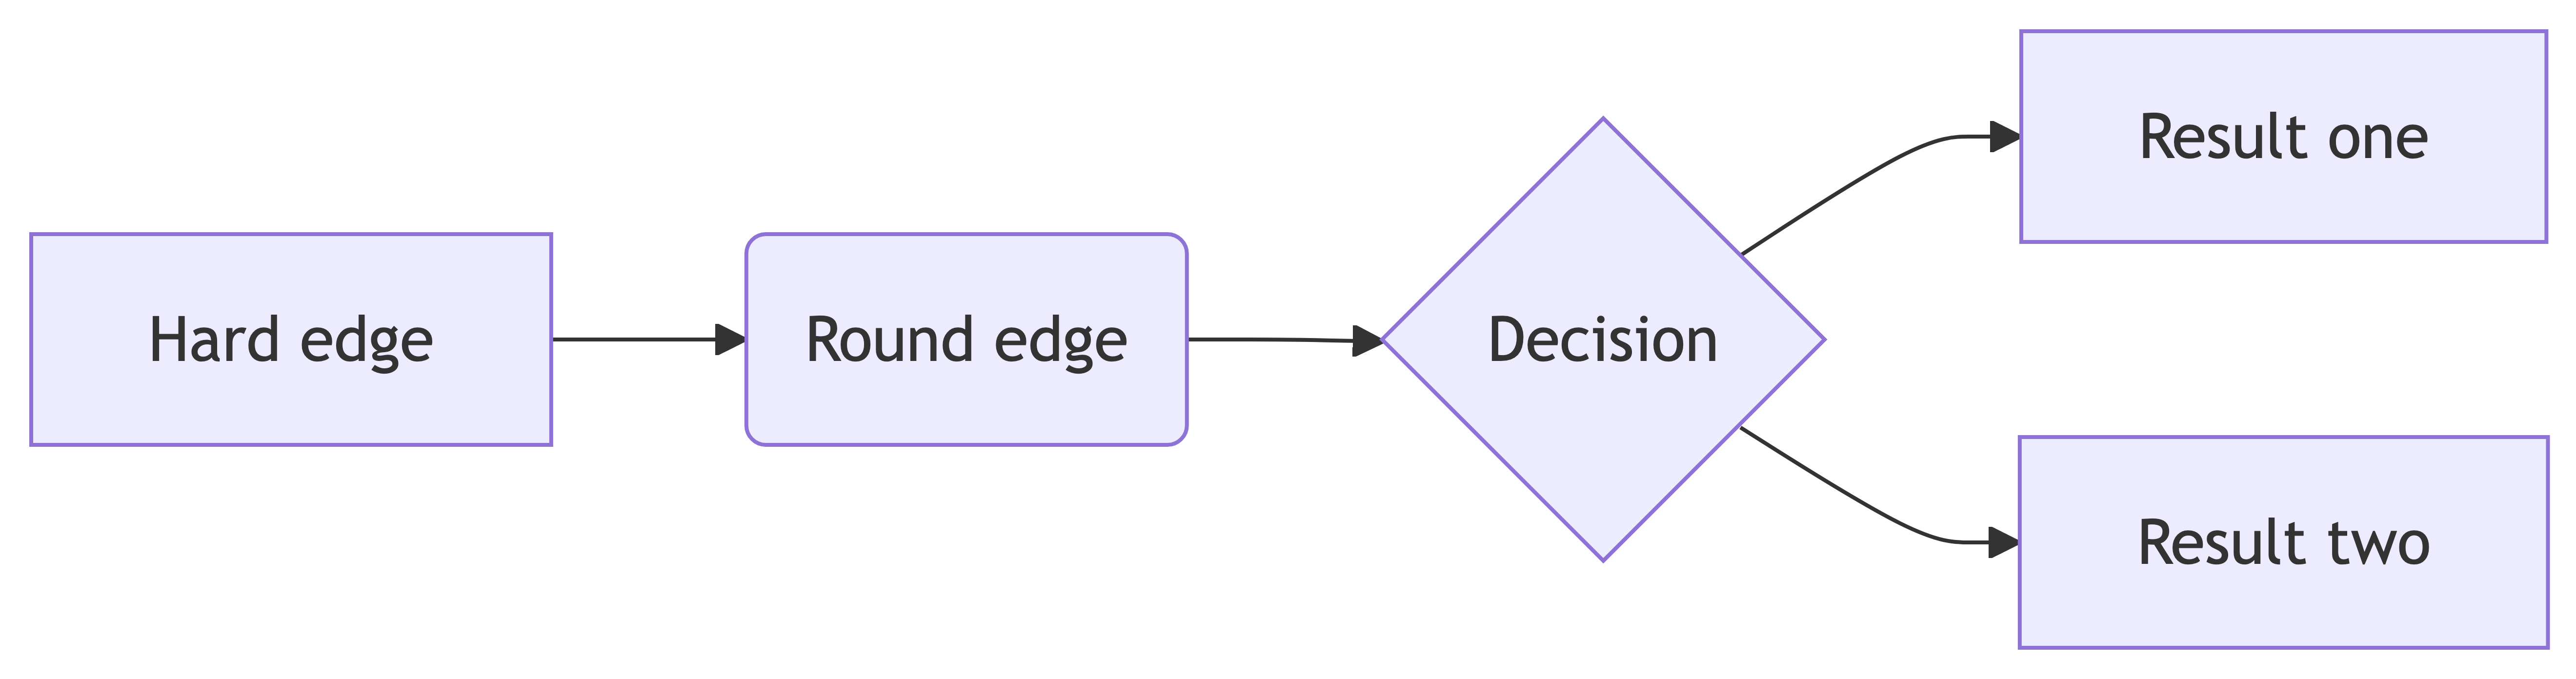
\includegraphics[width=6.88in,height=1.81in]{ref/references_files/figure-latex/mermaid-figure-2.png}

Testing crossreferencing grapics Figure~\ref{fig-automation_pipeline}.

\bookmarksetup{startatroot}

\chapter*{Bibliography (References)}\label{bibliography-references}
\addcontentsline{toc}{chapter}{Bibliography (References)}

\markboth{Bibliography (References)}{Bibliography (References)}

\phantomsection\label{refs}
\begin{CSLReferences}{1}{0}
\bibitem[\citeproctext]{ref-bucknall2022}
Bucknall, Benjamin S., and Shiri Dori-Hacohen. 2022. {``Current and
{Near-Term AI} as a {Potential Existential Risk Factor}.''} In
\emph{Proceedings of the 2022 {AAAI}/{ACM Conference} on {AI}, {Ethics},
and {Society}}, 119--29. Oxford United Kingdom: ACM.
\url{https://doi.org/10.1145/3514094.3534146}.

\bibitem[\citeproctext]{ref-growiec2024}
Growiec, Jakub. 2024. {``Existential Risk from Transformative {AI}: An
Economic Perspective.''} \emph{Technological and Economic Development of
Economy}, 1--27.

\bibitem[\citeproctext]{ref-knuth1984}
Knuth, Donald E. 1984. {``Literate Programming.''} \emph{Computer
Journal} 27 (2): 97--111. \url{https://doi.org/10.1093/comjnl/27.2.97}.

\bibitem[\citeproctext]{ref-soares2014}
Soares, Nate, and Benja Fallenstein. 2014. {``Aligning Superintelligence
with Human Interests: {A} Technical Research Agenda.''}

\end{CSLReferences}

\cleardoublepage
\phantomsection
\addcontentsline{toc}{part}{Appendices}
\appendix

\chapter{Appendices}\label{appendices-1}

\section{Appendix A: Technical Implementation
Details}\label{appendix-a-technical-implementation-details}

\section{Appendix B: Model Validation
Procedures}\label{appendix-b-model-validation-procedures}

\section{Appendix C: Case Studies}\label{appendix-c-case-studies}

\section{Appendix D: Ethical
Considerations}\label{appendix-d-ethical-considerations}

TestText

\chapter{appendixA}\label{appendixa}

testtext


\backmatter


\clearpage
\thispagestyle{empty} % Removes page numbering for current page

\newpage


% Top header with logo (left) and department (right)
\begin{minipage}{0.3\textwidth}
  
\includegraphics[width=5cm]{latex/uni-bayreuth-logo.png}
\end{minipage}
\hfill
\begin{minipage}{0.9\textwidth}
  \begin{center}
    -- P\&E Master's Programme --\\
    Chair of Philosophy, Computer\\
    Science \& Artificial Intelligence
  \end{center}
\end{minipage}

% Horizontal rule
\vspace{1.5cm}
\hrule
\vspace{2.5cm}

% Title in bold

  \LARGE\textbf{Affidavit}
\vspace{1.5cm}

\center

\normalsize

% \part*{Affidavit}

    \subsection*{\Large Declaration of Academic Honesty}
	    \vspace{1cm}\noindent \\
	    Hereby, I attest that I have composed and written the presented thesis 
        \vspace*{0.5cm}\noindent \\
        \textit{ \textbf{ Automating the Modelling of Transformative Artificial Intelligence Risks }}
        \vspace*{0.5cm}\noindent \\
        independently on my own, without the use of other than the stated aids and without any other resources than the ones indicated. All thoughts taken directly or indirectly from external sources are properly denoted as such.
	    \vspace{\baselineskip}
	    \\  This paper has neither been previously submitted in the same or a similar form to another authority nor has it been published yet.
	    \vspace{2cm}
	    
    \flushright
    \begin{minipage}{0.5\textwidth}
        \begin{flushleft} \large
        \textsc{Bayreuth}                     %   Place
        on the \\ % 26th of May 2025     \\
        \today           %   Date
        \vspace{2cm}\\
    	{\rule[-3pt]{\linewidth}{.4pt}\par\smallskip  
        \textsc{Valentin Meyer}	\\         %   Your name
    	}
        \end{flushleft}
        \end{minipage}


\end{document}
